\chapter{IJs, water, damp}\label{ch:g2:ice-water-steam}

Hetzelfde water dat als ijsblokje in je glas rinkelt, schenk je in als
drankje en stijgt als een witte pluim uit de soeppan op. Eén enkele
stof, drie \emph{toestanden}. Vorig jaar zagen we hoe warmte een
ijsblokje liet \omterm{def:g2:ice-water-steam:meltfreeze}{smelten}; dit jaar ontmoeten we alle drie de toestanden
die water kan aannemen.

\section{De drie toestanden van water}

\begin{example}[Waar elke toestand woont]\label{ex:g2:ice-water-steam:where}
Water kan in drie \emph{toestanden} voorkomen. \emph{Vast}: ijs ---
ijsblokjes, ijspegels onder de dakrand, rijp op het gras, sneeuw. Een
vaste stof is hard en houdt zijn vorm. \emph{Vloeibaar}: het water dat
stroomt --- regen, rivieren, de zee, je glas. Een vloeistof stroomt en
neemt de vorm van zijn beker aan. \emph{Gas}: waterdamp, water dat
onzichtbaar door de lucht vliegt. Vast, vloeibaar, gas --- maar
eronder altijd dezelfde stof.
\end{example}

\begin{omfigure}
\begin{tikzpicture}[scale=0.85]
  \draw[thick, omDef] (0.3,0.1) rectangle (1.5,1.3);
  \node[below, font=\small] at (0.9,-0.2) {ijs: vast};
  \draw[thick] (3.9,1.5) -- (4.2,0.1) -- (5.6,0.1) -- (5.9,1.5);
  \fill[omDef, opacity=0.25] (4.13,0.45) -- (5.67,0.45)
    -- (5.75,1.1) -- (4.05,1.1) -- cycle;
  \node[below, font=\small] at (4.9,-0.2) {water: vloeibaar};
  \draw[thick] (8.0,0.1) rectangle (10.4,1.0);
  \draw[thick] (10.4,0.75) -- (11.0,0.85);
  \foreach \x/\y in {8.6/1.35, 9.2/1.7, 9.8/1.4, 9.0/2.05} {
    \draw[omExo, thick] (\x,\y) circle (0.22);
  }
  \node[below, font=\small] at (9.2,-0.2) {waterdamp: gas};
\end{tikzpicture}

{\small Drie toestanden van één stof: het vaste ijsblokje, het
vloeibare glas vol, de pluim boven de pan die het gas verraadt.}
\end{omfigure}

\begin{remark}[Waterdamp is onzichtbaar]\label{rem:g2:ice-water-steam:invisible}
De witte pluim die je boven de pan ziet, bestaat uit piepkleine
zwevende waterdruppeltjes --- kleine druppels \emph{vloeistof}. Het
echte gas --- waterdamp, gemengd in de lucht --- is helemaal niet te
zien! Kijk goed naar de tuit van de pan: er vlak boven zit een kort
\emph{helder} stukje voordat de witte pluim begint. In dat stukje is
het water een gas, onzichtbaar; iets hoger klontert het samen tot de
druppeltjes die je wél ziet. In de lucht van elke kamer zit
onzichtbare waterdamp verstopt, en vóór het einde van dit hoofdstuk
betrappen we hem op heterdaad.
\end{remark}

\begin{omfigure}
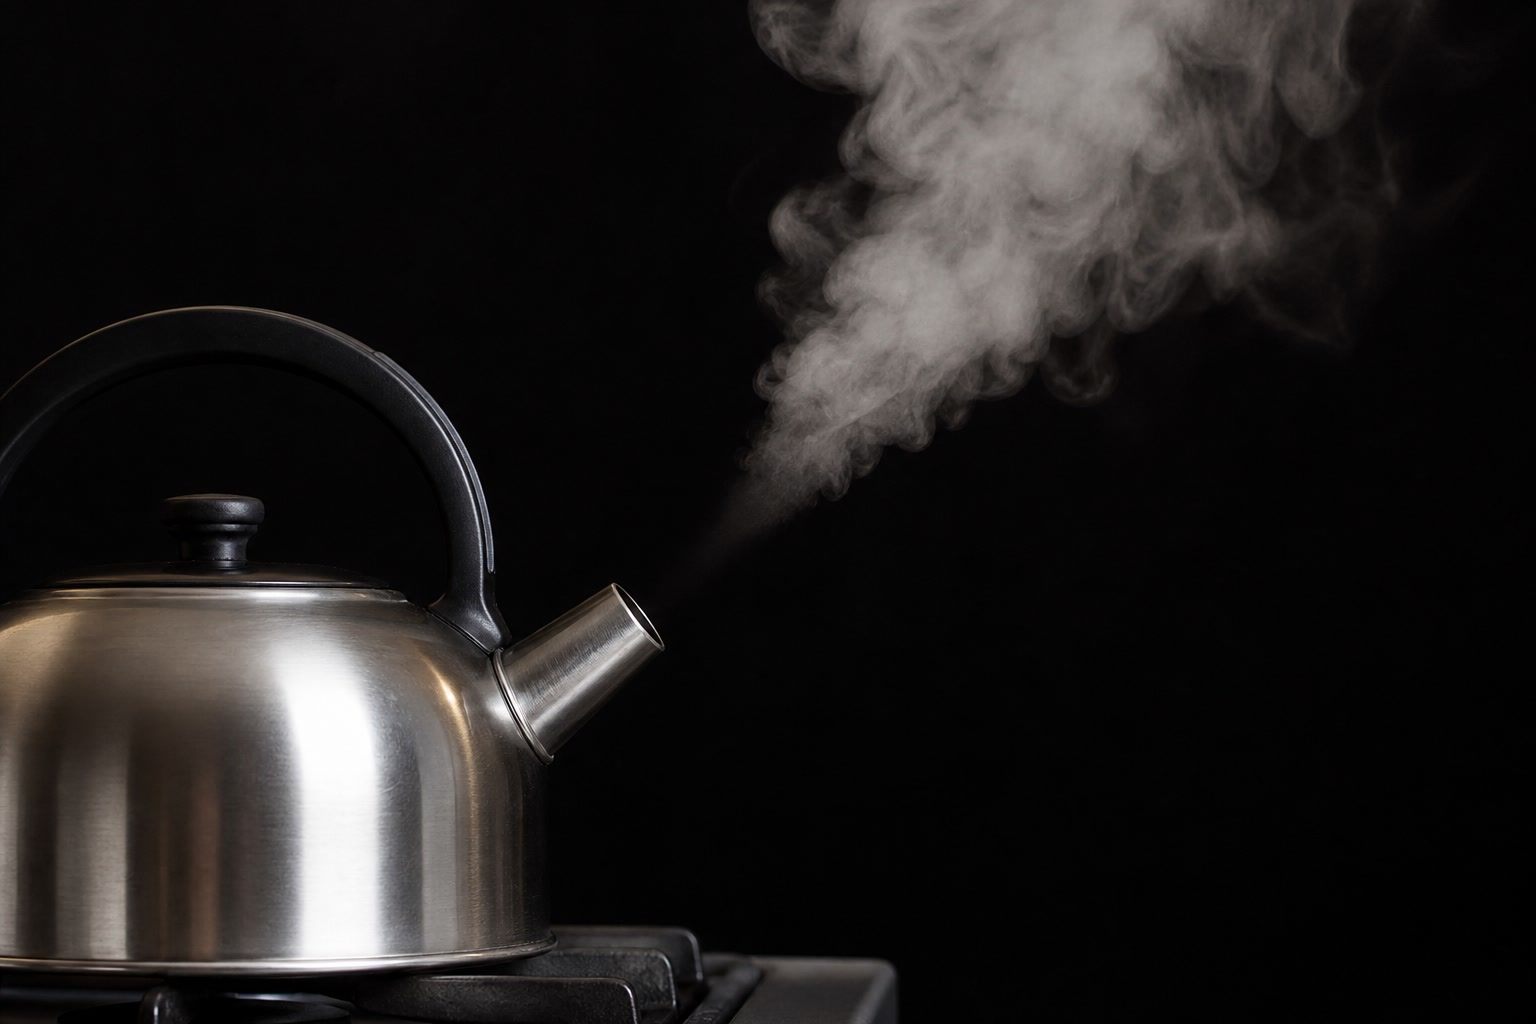
\includegraphics[width=0.55\linewidth]{images/book1/ai/g2-ice-water-steam-kettle.jpg}

{\small Het geheim van de waterkoker: vlak boven de tuit een kort \emph{helder} stukje waar het water een onzichtbaar gas is --- pas hoger \omterm{def:g2:ice-water-steam:evapcond}{condenseert} het tot de witte pluim die we kunnen zien.}
\end{omfigure}

\section{Van toestand veranderen}

\begin{definition}[Smelten en bevriezen]\label{def:g2:ice-water-steam:meltfreeze}
Als warmte vast ijs in vloeibaar water verandert, dan
\emph{smelt}\index{smelten} het ijs. Als strenge kou vloeibaar water
vast maakt, dan \emph{bevriest}\index{bevriezen} het water. Smelten en
bevriezen zijn tegenovergestelde deuren tussen dezelfde twee
toestanden: warmte duwt de ene kant op, kou de andere.
\end{definition}

\begin{definition}[Verdampen en condenseren]\label{def:g2:ice-water-steam:evapcond}
Als warmte vloeibaar water als gas de lucht in laat vliegen, dan
\emph{verdampt}\index{verdampen} het water --- de plas krimpt, de was
droogt. Als waterdamp iets kouds raakt en weer vloeibare druppeltjes
wordt, dan \emph{condenseert}\index{condenseren} hij --- wasem op het
koude raam, damp op de badkamerspiegel. Opnieuw twee
tegenovergestelde deuren: warmte stuurt water naar de gastoestand,
kou roept het terug naar de vloeistof.
\end{definition}

\begin{omfigure}
\begin{tikzpicture}[scale=0.85]
  \node[font=\small, draw, thick, omDef, minimum width=1.9cm,
    minimum height=0.85cm] (ice) at (0.8,0) {vast};
  \node[font=\small, draw, thick, omDef, minimum width=1.9cm,
    minimum height=0.85cm] (water) at (5.3,0) {vloeibaar};
  \node[font=\small, draw, thick, omDef, minimum width=1.9cm,
    minimum height=0.85cm] (steam) at (9.8,0) {gas};
  \draw[-Stealth, very thick, omThm] (1.85,0.28) -- (4.25,0.28);
  \node[above, font=\small, omThm] at (3.05,0.42) {warmte: smelten};
  \draw[-Stealth, very thick, omDef] (4.25,-0.28) -- (1.85,-0.28);
  \node[below, font=\small, omDef] at (3.05,-0.42) {kou: bevriezen};
  \draw[-Stealth, very thick, omThm] (6.35,0.28) -- (8.75,0.28);
  \node[above, font=\small, omThm] at (7.55,0.42) {warmte: verdampen};
  \draw[-Stealth, very thick, omDef] (8.75,-0.28) -- (6.35,-0.28);
  \node[below, font=\small, omDef] at (7.55,-0.42) {kou: condenseren};
\end{tikzpicture}

{\small De veranderingen van toestand: warmte duwt altijd naar rechts,
kou duwt altijd terug naar links.}
\end{omfigure}

\begin{example}[Probeer het: vang het onzichtbare water]\label{ex:g2:ice-water-steam:catch}
Pak een blikje of een glas zo uit de koelkast, droog de buitenkant
zorgvuldig af met een doek en zet het op tafel. Wacht terwijl je tot
$100$ telt. De buitenkant beslaat en wordt dan nat --- er verschijnen
druppels uit het niets! Ze lekken niet door het glas heen: de
onzichtbare waterdamp in de lucht van de kamer raakte de koude wand en
condenseerde. Je hebt zojuist het onzichtbare gas gevangen.
\end{example}

\begin{example}[Wolkjes uit je mond]\label{ex:g2:ice-water-steam:breath}
In je adem zit altijd onzichtbare waterdamp. Op een warme dag blijft
die onzichtbaar. Op een vrieskoude ochtend \omterm{def:g2:ice-water-steam:evapcond}{condenseert} de koude
buitenlucht hem meteen tot een wolkje voor je mond --- en hetzelfde
gebeurt op een koud raam als je erop blaast om met je vinger te
tekenen.
\end{example}

\begin{remark}[Damp en fornuis: voorzichtig]\label{rem:g2:ice-water-steam:safety}
De waterdamp boven een kokende pan is gloeiend heet --- heter dan het
water zelf aanvoelt. Steek je hand nooit in de pluim, en til deksels
van je af, met een volwassene in de buurt. Veranderingen van toestand
zijn om naar te kijken, niet om aan te raken, zodra er een fornuis aan
te pas komt.
\end{remark}

\section{Hetzelfde water, rondje na rondje}

\begin{example}[De krimpende plas]\label{ex:g2:ice-water-steam:puddle}
Na de regen glimt er een plas op het schoolplein. 's Middags is hij
gekrompen; morgen is hij weg. Niemand heeft hem opgedronken en hij is
niet door het asfalt gelekt: de warmte van de Zon liet hem druppel
voor druppel \omterm{def:g2:ice-water-steam:evapcond}{verdampen} in de lucht. Trek 's ochtends met krijt een
lijn om een plas en kijk na de lunch: het water heeft zich
teruggetrokken binnen je lijn.
\end{example}

\begin{example}[Van de zee naar de regen]\label{ex:g2:ice-water-steam:cycle}
Wat \omterm{def:g2:ice-water-steam:evapcond}{verdampt} moet ergens \omterm{def:g2:ice-water-steam:evapcond}{condenseren}. Water vliegt onzichtbaar
omhoog uit zeeën en plassen; hoog in de lucht, waar het koud is,
\omterm{def:g2:ice-water-steam:evapcond}{condenseert} het tot de druppeltjes waaruit wolken bestaan; de
druppeltjes klonteren samen, worden zwaar en vallen --- regen! De
regen vult de plassen en de zeeën, en de rondreis begint opnieuw. Het
water in jouw glas heeft die reis vaker gemaakt dan iemand kan tellen.
\end{example}

\section{Oefeningen}

\begin{exercise}[$\star$]\label{exo:g2:ice-water-steam:1}
In welke toestand verkeert elk van deze --- vast, vloeibaar of gas:
een ijspegel; \ de zee; \ het onzichtbare water vlak boven de tuit van
de soeppan; \ rijp op het gras; \ regen?
\end{exercise}

\begin{exercise}[$\star$]\label{exo:g2:ice-water-steam:2}
Noem de verandering van toestand: een sneeuwpop die in de zon krimpt;
\ een plas die verdwijnt; \ wasem die op de badkamerspiegel verschijnt;
\ een vijver die 's winters hard wordt.
\end{exercise}

\begin{exercise}[$\star$]\label{exo:g2:ice-water-steam:3}
Welke kant duwt warmte in de tekening van de toestandsveranderingen
altijd op: naar het vaste of naar het gas? En kou?
\end{exercise}

\begin{exercise}[$\star$]\label{exo:g2:ice-water-steam:4}
De druppels op het koude blikje van \cref{ex:g2:ice-water-steam:catch}
--- zijn die door het glas naar buiten gelekt? Waar kwamen ze vandaan?
\end{exercise}

\begin{exercise}[$\star$]\label{exo:g2:ice-water-steam:5}
Waarom zie je je adem op een vrieskoude ochtend wel en op een warme
dag niet? Gebruik de woorden van \cref{def:g2:ice-water-steam:evapcond}.
\end{exercise}

\begin{exercise}[$\star$]\label{exo:g2:ice-water-steam:6}
Natte was droogt sneller in de zon dan in de \omterm{def:g1:light-and-shadows:shadow}{schaduw}. Welke
verandering van toestand is aan het werk, en wat voegt de Zon toe om
haar te versnellen?
\end{exercise}

\begin{exercise}[$\star$]\label{exo:g2:ice-water-steam:7}
Waarom is de pluim boven een kokende pan gevaarlijk, en wat is de
veilige regel uit \cref{rem:g2:ice-water-steam:safety}?
\end{exercise}

\begin{exercise}[$\star$]\label{exo:g2:ice-water-steam:8}
Vertel de rondreis van een regendruppel: begin bij de zee, eindig weer
in de zee, en gebruik onderweg de woorden \omterm{def:g2:ice-water-steam:evapcond}{verdampen} en
\omterm{def:g2:ice-water-steam:evapcond}{condenseren}.
\end{exercise}

\begin{exercise}[$\star\star$]\label{exo:g2:ice-water-steam:9}
Boven de tuit van de pan zit een helder stukje, en pas daarboven
begint de witte pluim. Wat zit er in dat heldere stukje? Wat laat dat
zien over water in de gastoestand?
\end{exercise}

\begin{exercise}[$\star\star$]\label{exo:g2:ice-water-steam:10}
Nino laat een glas water een week op de vensterbank staan; het niveau
zakt dag na dag, terwijl niemand ervan drinkt. Zijn kat wordt
beschuldigd. Verdedig de kat: leg uit wat er werkelijk is gebeurd, en
verzin een manier om te laten zien dat het water \emph{de lucht in}
verdwijnt en niet in de kat.
\end{exercise}
